Le misure effettuate per questo progetto sono state eseguite su una macchina con le seguenti caratteristiche:
\begin{itemize}
	\item Processore: AMD ryzen 7 5700G (8 core, 16 thread, 3.8 GHz)
	\item RAM: 32 GB DDR4 3200 MHz
	\item Sistemi operativi: Windows 11 25H2 e Linux Fedora 44
	\item Linguaggi di programmazione: C++ e Matlab
	\item Dischi: SSD NVMe 
\end{itemize}
\section{Matlab}
Per quanto riguarda Matlab, abbiamo utilizzato la versione R2025b.
Per la risoluzione dei sistemi di equazioni è stato utilizzato il comando \texttt{mldivide}, che implementa una serie di controlli per scegliere il metodo più adatto a seconda del tipo di matrice (densa, sparsa, simmetrica, ecc.).
\begin{figure}
	\centering
	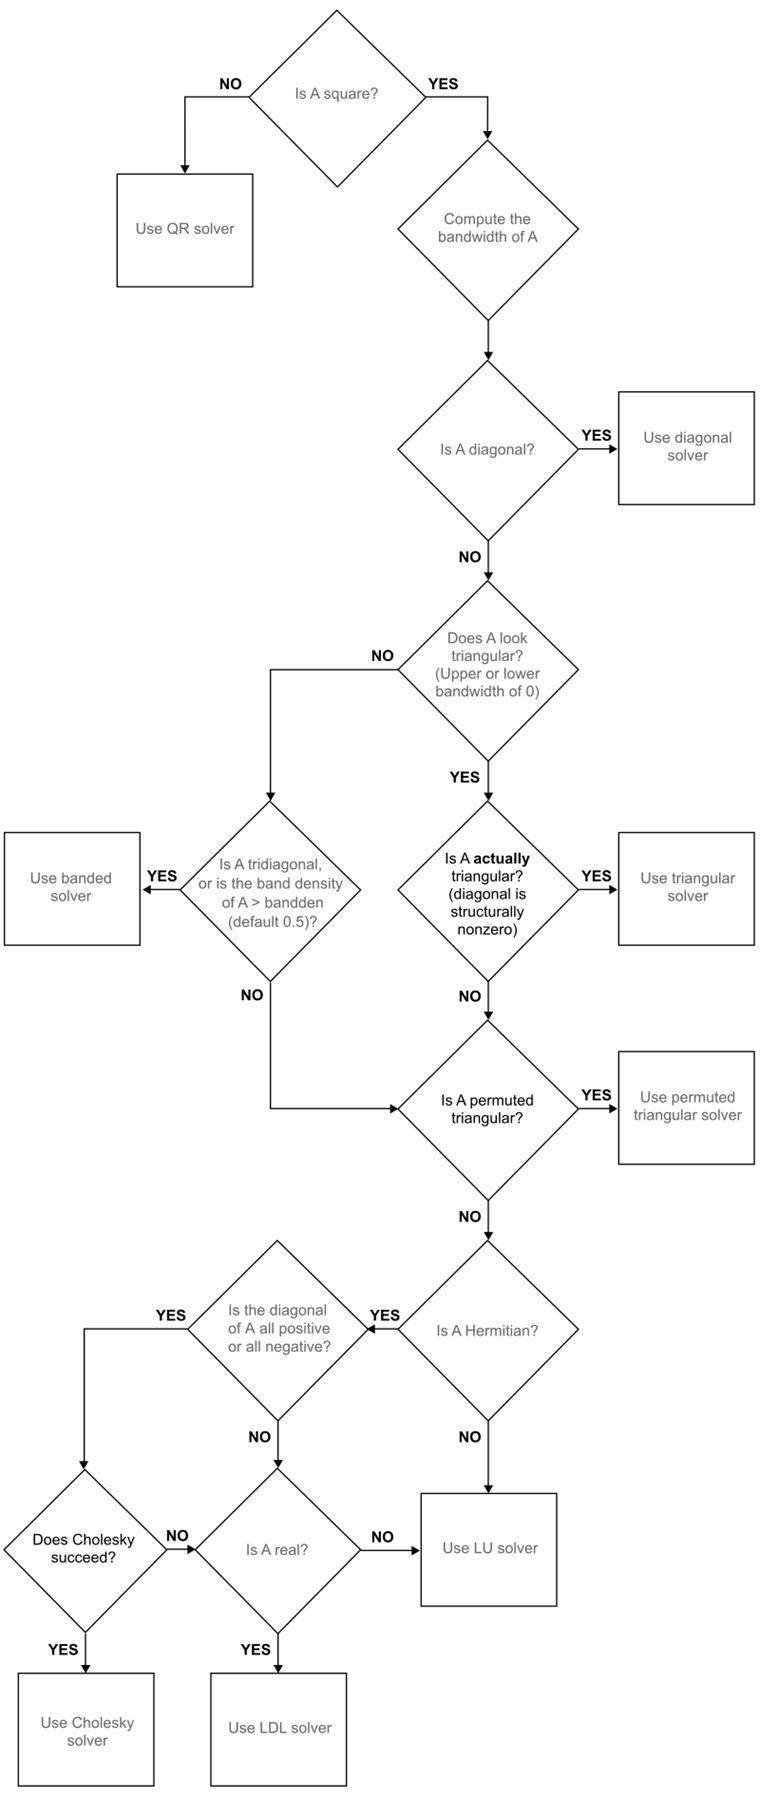
\includegraphics[height=0.95\textheight]{figures/mldivide_sparse.png}
	\caption{Scelta del metodo di risoluzione in Matlab per matrici sparse di \texttt{mldivide} \cite{noauthor_mldivide_nodate}.}
	\label{fig:mldivide_sparse}
\end{figure}
Questa libreria viene mantenuta e aggiornata regolarmente da MathWorks, ottimizzando i metodi di risoluzione per alcuni tipi di matrici	e migliorando le prestazioni complessive.
La documentazione ufficiale di Matlab fornisce i dettagli sulla selezione del metodo di risoluzione in base alle caratteristiche della matrice, dividendo in due macro categorie: matrici dense e matrici sparse.
In particolare, in figura~\ref{fig:mldivide_sparse} possiamo vedere il processo di selezione del metodo di risoluzione per matrici sparse, che è quello che abbiamo utilizzato per i nostri benchmark.
\section{C++}
Per quanto riguarda C++, abbiamo scelto di utilizzare la libreria \texttt{Eigen}, la quale mette a disposizione
una vasta gamma di funzioni per l'algebra lineare, come per la manipolazione di matrici e vettori oppure per la risoluzione
di sistemi di equazioni lineari.
Eigen permette inoltre di interfacciarsi con diversi moduli esterni per la risoluzione  di sistemi di equazioni lineari, come, ad esempio, il pacchetto SuiteSparse,
il quale è stato utilizzato per i benchmark presentati in questo report.
In particolare, abbiamo utilizzato la libreria \texttt{CHOLMOD} di SuiteSparse, la quale offre un metodo di risoluzione tramite fattorizzazione di Cholesky più efficiente rispetto al risolutore standard con metodo di Cholesky offerto da Eigen \cite{eigen_simpicial_llt}. 
L'interfaccia di Eigen per \texttt{CHOLMOD}, contenuta nel modulo \texttt{CholmodSupport} \cite{cholmod_eigen}, permette di sfruttare le diverse funzionalità offerte dalla libreria.
\subsubsection{CHOLMOD}
\texttt{CHOLMOD} è una libreria che permette di svolgere efficientemente diverse operazioni su matrici sparse.
In particolare, la libreria offre funzioni per la fattorizzazione di matrici sparse, simmetriche e definite positive
tramite il metodo di Cholesky e per la risoluzione di sistemi lineari. La libreria è scritta nel linguaggio di programmazione C.
Sia $A$ una matrice sparsa, simmetrica e definita positiva; allora la sua decomposizione ottenuta usando il metodo di Cholesky è $A = LL^T$,
con $L$ una matrice triangolare inferiore. 
\texttt{CHOLMOD} implementa due tipi di risolutori di sistemi di equazioni lineari sparsi che sfruttano questa decomposizione:
uno \textbf{supernodale} e uno \textbf{non-supernodale} \cite{chen_algorithm_2008}.
In particolare, abbiamo scelto di utilizzare l'implementazione \textbf{supernodale} dell'algoritmo di risoluzione, il quale è accessibile in Eigen costruendo un risolutore della classe \texttt{CholmodSupernodalLLT}\cite{supernodal_chol_eigen}.
%Informalmente, data le decomposizione di Cholesky $A = LL^T$, un \textbf{supernodo} è un insieme di colonne adiacenti di $L$ aventi un pattern identico di entrate non nulle.
%I supernodi sono tipicamente immagazzinati in memoria in modo tale da sfruttarne la struttura, come, per esempio, in matrici dense di dimensioni $s \times z$, dove
%$s$ è il numero di entrate non nulle nella prima colonna del supernodo e $z$ è il numero di colonne nel supernodo \cite{davis_dynamic_2009}.
Gli algoritmi supernodali si basano sulla decomposizione della matrice $A$ in termini di blocchi di colonne, chiamati \textbf{supernodi}. L'algoritmo implementato da CHOLMOD è composto da tre fasi di calcolo principali:
\begin{enumerate}
	\item La prima analizza la struttura della matrice e riordina le righe e le colonne per minimizzare il fill-in, ovvero l'introduzione di elementi non-nulli in $L$ che non compaiono nella posizione corrispondente in $A$.
	Il riordinamento della matrice è un'importante fattore di performance, dato che con meno valori non nulli il numero di operazioni necessario e il peso in memoria diminuisce.
	\item La seconda fase fattorizza la matrice applicando operazioni sui supernodi
	\item La terza risolve due sistemi triangolari di equazioni: $Ly = b$ e $L^T x = y$ nel caso della fattorizzazione di Cholesky.
\end{enumerate}
Tra le tre fasi, quella di fattorizzazione rappresenta la parte computazionalmente più onerosa del risolutore implementato da CHOLMOD \cite{le_fevre_selective_2022}.
Per sfruttare al meglio le moderne architetture delle CPU multicore, \texttt{CHOLMOD} utilizza la libreria \texttt{Open MultiProcessing (OpenMP)} \cite{cholmod_doc} per implementare la parallelizzazione di alcune delle operazioni necessarie alla risoluzione del sistema di equazioni lineari,
permettendo quindi di sfruttare al meglio la CPU e, agli scopi del benchmark, ottenere un confronto più equo con Matlab.
Infine, \texttt{CHOLMOD} dipende inoltre da diverse librerie per effettuare i calcoli necessari alla decomposizione e alla risoluzione del sistema di equazioni lineari:
\begin{itemize}
	\item \textbf{Librerie per l'ordinamento della matrice}: Per effettuare l'ordinamento della matrice nella prima fase dell'algoritmo di risoluzione, \texttt{CHOLMOD} può utilizzare diversi algoritmi, come \textit{Approximate Minimum Degree ordering} e \texttt{METIS} \cite{le_fevre_selective_2022}.
	Per questo motivo, \texttt{CHOLMOD} dipende dalle librerie di SuiteSparse \texttt{AMD, CAMD, COLAMD, CCOLAMD} e \texttt{METIS}.
	\item \textbf{Basic Linear Algebra Subroutines (BLAS)}: BLAS \cite{blas_doc} è un insieme di specifiche open per l'implementazione di funzioni a basso livello per svolgere le comuni operazioni richieste per l'algebra lineare.
	Esistono diverse implementazioni delle funzioni descritte da BLAS, tra cui \textbf{OpenBLAS} e \textbf{FlexiBLAS}, entrambe utilizzate per i benchmark presentati in questo report.
	\item \textbf{Linear Algebra PACKage (LAPACK)}: LAPACK \cite{lapack_doc} è una libreria che offre diverse funzioni per la risoluzione di sistemi lineari. La libreria dipende dalla presenza di un'implementazione di BLAS ed è scritta
	in modo tale che la computazione sia svolta effettuando il più possibile chiamate alle funzioni offerte dall'implementazione di BLAS sottostante.
\end{itemize}
\section{Windows}

\section{Linux}












